\documentclass[times, utf8, diplomski]{fer}
\usepackage{booktabs}
\usepackage[utf8]{inputenc}

\usepackage[T1]{fontenc}
\usepackage{fixltx2e}
\usepackage{graphicx}
\usepackage{longtable}
\usepackage{float}
\usepackage{wrapfig}
\usepackage{soul}
\usepackage{textcomp}
\usepackage{marvosym}
\usepackage{wasysym}
\usepackage{latexsym}
\usepackage{amssymb}
\usepackage{hyperref}
\usepackage{caption}
\usepackage[usenames, dvipsnames]{color}

\begin{document}

\title{LISA}

\author{Filip Paveti\'{c}, Goran \v{Z}u\v{z}i\'{c}}

\maketitle

% Dodavanje zahvale ili prazne stranice. Ako ne želite dodati zahvalu, naredbu ostavite radi prazne stranice.
\zahvala{}

\tableofcontents

\chapter{Uvod}
Ovaj rad opisuje sustav za mapiranje kratkih DNA sekvenci na referentni genom. Rad je podijeljen na 4 dijela:
\begin{itemize}
\item u prvom dijelu ćemo napraviti kratki uvod u probleme bioinformatike i pozadinu problema kojeg sustav rješava
\item drugi dio se bavi modelom, algoritmom i implementacijom nad kojim je sustav ostvaren
\item slijede rezultati testiranja i usporedba s najpoznatijim analognim alatima
\item naposlijetku dajemo kratki zaključak i smjernice za daljnji rad
\end{itemize}

Sustav je razvijen u sklopu natjecanja identifikacija organizama iz toka DNA sekvenci
kojeg je objavila tvrtka \emph{InnoCentive} pod sponzorstvom vlade Sjedinjenih Američkih Država
i koje još nije završilo \footnote{više informacija o samom natjecaju možete pronaći na \emph{http://tinyurl.com/dna-dtra}}.

\section{Bioinformatika}

Bioinformatika je u posljednjih nekoliko godina u centru ogromne pažnje i entuzijazma do kojih su
doveli napretci u razumijevanju živih bića i brzom razvoju tehnologije pomoću kojih ih možemo proučavati.
Dosada se bioinformatika koristila u svrhe proučavanja nasljednih svojstava, evolucije između vrsta i identifikacije
patogenih bakterija, dok se u bliskoj budućnosti vjeruje kako će pomoći u proizvodnji boljih lijekova koji bi bili
posebno prilagođeni zaraženoj osobi.

Molekularna biologija i biokemija su nam otkrili kako najveću funkcionalnu ulogu u gotovo svim biološkim procesima
živih organizama imaju molekule zvane \emph{proteini}, linearni nizovi aminokiselina spojenih peptidnim vezama.
Njihova uloga u organizmima seže od katalizacije procesa (npr. kod metabolizma), signalizacije i adhezije stanica
sve do imunološkog sustava. Proteini su konstruirani zasebno u svakoj stanici od svojih gradivnih elemenata (aminokiselina),
a kod koji specificira način na koji se grade proteini se nalazi u masivnoj staničnoj molekuli
deoksiribonukleinske kiseline (DNA).

Dominantno područje bioinformatike se bavi sekvenciranjem (čitanjem) i analizom DNA. Molekula DNA je dugi linearni niz sastavljen od otprilike
3 milijarde\footnote{kod ljudi} povezanih parova baza nukleinskih kiselina. Veličina tih brojeva stvara potrebu za razvojem računalnih alata
bez kojih bilo kakva obrada postaje nemoguća.

Nedavni razvoj moderne tehnologije je doveo do strmoglavog pada cijene sekvenciranja molekule DNA do te razine da je
postalo jasno kako će u bliskoj budućnosti najsporiji i najteži dio bioinformatike biti u konstrukciji efikasnih
algoritama koji brzo i pouzdano obrađuju sve veču i veću količinu informacija na njihovom raspolaganju.

\section{DNA i mutacije}
Kao što je spomenuto, DNA modeliramo kao linearni niz povezanih parova baza. U DNA se pojavljuju točno četiri različite baze i njih
označavamo slovima \emph{A, G, T} i \emph{C}\footnote{skraćeno od adenin, guanin, timin i citozin, vrsta nukleinskih kiselina koje se pojavljuju}.
Na taj način DNA modeliramo dugim nizom slova nad gornjom četvoroslovnom abecedom, primjerice:

\begin{verbatim}
... AGTGAGGAAAAAAAAAGGTCAATGCAGCACTTGAGCCAACATTGTAGAT
    GTTGTACTGCAAGGTCAGGTCTCGCCCCTCCACGGCGTATCTGTTCAG
    CAGTGACTTGGAGGCAAGAAAATCAAACCCGTGATCGATGGTACCGAGC ...
\end{verbatim}

Kroz vrijeme se na molekuli DNA javljaju razne mutacije. Okvirno poznavanje mogućih mutacija je nužno za bolje razumijevanje izazova koji se javljaju u bioinformatici. Biolozi su izolirali nekoliko dominantnih mutacija:

\begin{enumerate}
\item Supstitucija - zamjena jedne baze drugom. Najčešća od navedenih mutacija.
  Uzrokovana greškama u replikaciji i kemikalijama.
  \nopagebreak
  \begin{figure}[!ht]
    \begin{center}
      A C G \textcolor{blue}{T} T G A C \\
      A C G \textcolor{red}{A} T G A C
      \caption{Primjer supstitucije}
    \end{center}
  \end{figure}

\item Ispuštanje i umetanje - iz DNA se ukloni ili doda slijed baza. Ova mutacija je vrlo štetna i obično
  rezultira gubitkom funkcionalnosti tog dijela gena.

  \nopagebreak
  \begin{figure}[!ht]
    \begin{center}
      A C G \textcolor{red}{T T G} A C \\
      A C G A C
      \caption{Primjer ispuštanja}
    \end{center}
  \end{figure}
\item Udvostručavanje - ponavljanje dijela sekvence dva ili više puta zaredom. Ova mutacija je iznimno rijetka,
  ali se smatra da je unatoč tomu imala veliku ulogu u povećanju genetskog koda živih bića.
  \begin{figure}[!ht]
    \begin{center}
      A C G \textcolor{blue}{T T G A} C \\
      A C G \underline{\textcolor{red}{T T G A}} \underline{\textcolor{red}{T T G A}} C \\
      \caption{Primjer udvostručavanja}
    \end{center}
  \end{figure}
  
\item Inverzija - okretanje dijela sekvence. Iznimno rijetka mutacija koja se najčešće zanemaruje pri analizi.
  \begin{figure}[!ht]
    \begin{center}
      A C \textcolor{blue}{T C A A} G G \\
      A C \textcolor{red} {A A C T} G G
      \caption{Primjer inverzije}
    \end{center}
\end{figure}
\end{enumerate}

\section{Sekvenciranje DNA}

Prvi pokušaj sekvenciranja ljudskog DNA počinje 1990. s američkim \emph{Human Genome Project} koji je trajao 15
godina i uspješno identificirao većinu ljudskog genoma. Ukupna cijena projekta je procijenjena na \$3.000.000.000.
(TODO: referenca)
Od tada cijena sekvenciranja DNA strmoglavo pada i očekuje se će u sljedećih nekoliko godina dostići \$1.000 za
cjelokupni ljudski genom.

Sekvenciranje DNA se odvija u nekoliko faza: (1) prikupljanje kratkih očitanja, (2) poravnavanje s referentnim genomom, (3) izlistavanje varijanti i (4) filtriranje i označavanje.

\begin{description}
\item[Prikupljanje kratkih očitanja] je biološki dio sekvenciranja tijekom kojeg se DNA višestruko replicira puta, slučajno lomi na dijelove duljine 100-3000 baza te se potom očitava složenim metodama. Te metode su podložne pogreškama uslijed krivog čitanja dijela sekvenci, gubljenja informacija i dvosmislenosti podataka koji se javljaju tijekom loma.

\item[Poravnavanje s referentnim genomom] je proces mapiranja kratkih očitanja na referentni genom. Uobičajeni volumen podataka od otprilike desetke milijuna očitanja i tri milijarde startnih pozicija čini ovaj posao vrlo
algoritamski zahtjevnim. Još kritičnim ovaj korak čini svojstvo da se sve greške na ovom koraku propagiraju i
ruše kvalitetu svim preostalim dijelovima sekvenciranja.

\item [Izlistavanje varijanti] je korak u kojem se uspoređuju poravnata očitanja s referentnim genomom. Pronađene
mutacije mogu biti uzročnici nasljednih bolesti ili mogu jednostavno biti genski šum bez funkcionalnih svojstava.

\item [Filtriranje i označavanje] procjenjuje koja od potencijalnih razlika između interesantnih gena pridonosi 
patološkom procesu kojeg proučavamo. Filtriraju se mutacije bez funkcionalnih značajki te se propoznaju česte prisutne populacijske mutacije.
\end{description}

\section{Obrazloženje teme}

Izgrađeni sustav se bavi problematikom \emph{poravnavanja očitanja s referentnim genomom}. Specifično, potrebno
je za svaki od nekoliko desetaka milijuna očitanja koja su skupljena u FASTQ datoteku mapirati na poziciju u
referentnom genomu. Problem su pritom gore opisane mutacije, pogreške u kratkim očitanjima, dvosmisleni podaci,
regije niske složenosti te repetitivne regije koje se mogu mapirati na više mjesta u referentnom genomu.

Ovaj sustav se koristi kao prvi korak prilikom rješavanja problema identifikacije organizama iz toga DNA sekvenci
koji se pojavio na natjecanju sponzoriranom od strane vlade Sjedinjenih Američkih Država. Autori ovog rada sudjeluju
na tome natjecanju u sklopu tima Fakulteta elektrotehnike i računarstva Sveučilišta u Zagrebu.




\chapter{Pristup}

\section{Pregled}
Ovo poglavlje počinjemo kratkih pregledom trendova u razvoju mappera te kasnije dajemo detaljan opis našeg pristupa. Jedan od prvih algoritama za poravnanje očitanja je algoritam globalnog poravnanja pod nazivom Smith-Waterman (TODO referenca). Rješenje dobiveno tim algoritmom može se smatrati veoma točnim zbog toga što ima statistički opravdano značenje, međutim zbog velike vremenske složenosti algoritma (TODO napisati složenosti) nije praktično za korištenje.\\
Većina boljih modernih mappera (poput SNAP-a (TODO referenca) i SeqAlto-a (TODO referenca)) koriste tkzv. seed-and-extend pristup. U tom pristupu prvo se od referentnog genoma gradi indeks koji mapira niz od svakih uzastopnih k-znakova genoma na sve pozicije unutar genoma na kojima se taj podniz nalazi. Ukupan broj takvih različitih podnizova je $4^k$, što je i prva praktična opaska, jer za $k\le32$ možemo takav podniz zakodirati u $64$-bitni cjelobrojni tip podataka. Očitanja se obrađuju na način da se ponovno promatraju podnizi uzastopnih znakova duljine $k$ te se vrši upit u prethodno izgrađeni indeks. Pozicije dobivene takvim upitom daju kandidatne pozicije u čijoj se okolini nalazi potencijalno poravnanje očitanja na genom. Razlike između mappera ovog tipa su primarno u načinu izgradnje indeksa i načinu ocjene kvalitete poravnanja na nekoj kandidatnoj poziciji. Tako primjerica SNAP koristi hash tablicu kao strukturu podataka nad kojom je izgrađen indeks, dok SeqAlto koristi sortirano polje. Za ocjenu kvalitete SNAP koristi \emph{edit-distance} metriku, dok SeqAlto koristi općenitiju \emph{Needleman-Wunsch} metriku. Oba pristupa daju značajno poboljšanje efikasnosti u odnosu na pristup spomenut na početku ove sekcije, međutim ti su mapperi i dalje nepraktični budući da kroz vrijeme strojevi za izradu očitanja napreduju i duljine očitanja postaju sve veće čime pretpostavke koje osiguravaju efikasnost ovih alata postaju prejake (glavni razlog je što u njihovim implementacijama izračun tih metrika ima vremensku složenost linearno proporcionalno s duljinama očitanja).\\
Naš mapper indeks izgrađuje po uzoru na SeqAlto, međutim uvodimo novu metriku ocjene kvalitete koja za red složenosti poboljšava postojeće algoritme bez gubitka točnosti što ćemo potkrijepiti eksperimentima u kasnijim poglavljima.
Metrika kvalitete bazira se na traženju najduljeg uzlaznog podniza\footnote{engl. Longest Increasing Subsequence; odatle dolazi inspiracija za naziv LISA - LIS Aligner}\\

\section{Opis pristupa}

Glavna inspiracija prema našem algoritmu dolazi iz nekoliko činjenica. Prvo, za malu količinu grešaka (to je realan slušaj, očitanja s velikim postotkom greške nisu korisna za ikakve zaključke) unutar očitanja postojat će mnogo nizova uzastopnih znakova koji nisu dotaknuti greškom. Mi želimo iskoristiti tu činjenicu pa dizajniramo algoritam koji nastoji poravnati dijelove netaknute greškom, a one koji je sadrže ignorira. Pokazuje se da je za veće duljine očitanja ovaj pristup iznimno uspješan\footnote{Trenutna pretpostavka koju radimo je da dugačka očitanja imaju svoje jedinstveno mjesto u genomu. Neki drugi mapperi ne rade tu pretpostavku pa je u daljnjim planovima razvoja LISA-e dopustiti mogućnost poravnanja na više različitih mjesta unutar genoma.}

TODO: slika koja stavlja read ispod genoma i dočarava prianjanje

\subsection{Indeks}
U pregledu poglavlja spomenuli smo da za izgradnju indeksa pratimo smjernice SeqAlto mappera. Svaki niz $i$ od $k=20$ uzastopnih znakova na poziciji $p_i$ unutar genoma kodiramo jednim cijelim brojem $h_i$ koji predstavlja hash bez kolizije. Indeks nam čini polje uređenih parova $(h_i, p_i)$. To je polje sortirano pa koristimo binarno pretraživanje kako bi dohvat pozicija za neki zadani hash bio efikasan. Dodatno, one $h_i$-ove koji se pojavljuju jako velik broj puta njihove parove mičemo iz niza jer takvi ne donose korisnu informaciju, a samo povećavaju vremensku i memorijsku složenost. 

TODO: neka slika koja reprezentira DNA+indeks 

\subsection{LISA algoritam poravnanja}
Algoritam poravnanja sastoji se od dva koraka:
\begin{enumerate}
\item Grubo određivanje pozicije očitanja unutar genoma
\item Fino određivanje pozicije očitanja unutar genoma
\end{enumerate}

\subsubsection{Grubo određivanje pozicije očitanja}

U ovoj baznoj fazi algoritma poravnanja određujemo poziciju unutar genoma oko koje je očitanje koncentrirano. Opća ideja iza algoritma je konstrukcija niza brojeva (kojeg ćemo uskoro opisati) nad kojim pokrećemo algoritam nalaženja najduljeg rastućeg podniza\footnote{Algoritam je opisan u Dodatku}. Nađeni podniz ugrubo opisuje poziciju poravnanja i koristi se u sljedećoj fazi za traženje točne pozicije poravnanja.\\
Potreban niz $P$ konstruiramo tako da promatramo sve nizove uzastopnih znakova $i$ duljine $k$ unutar očitanja s lijeva na desno. Za svaki od njih vršimo upit za pozicije unutar kojih se nalazi u indeksu. Na kraj niza $P$ za svaku od dobivenih pozicija $x$ dodajemo par $(x,i)$. Kada smo to ucinili za sve nizove $i$, sortiramo $P$ po prvom broju u paru i pokrecemo algoritam pronalaska najduljeg zajedničkog podniza $L$ nad nizom drugih brojeva parova u $P$. $L$ koristimo u sljedećoj fazi. Pseudokod algoritma dan je u TODO: pseudokod.

\subsubsection{Fino određivanje pozicije očitanja}

Razlog zašto je ova faza potrebna je vidljiv na TODO: dodati sliku. Očito je da je pravo poravnanje smješteno oko pozicije TODO: pozicija, dok bismo pogrešnom naivnom procjenom možda rekli da je ono ipak TODO: pozicija. Pseudokod TODO: pseudokod jednostavno opisuje rad ove faze.

\subsubsection{Mjera pouzdanosti}

Mjerenje pouzdanosti je još uvijek otvoren problem za LISA-u. Trenutno koristimo omjer duljine pronađenog rastućeg niza i duljine očitanja.

\chapter{Implementacija}

Implementacija sustava može biti vrlo prirodno razložena na dva osnovna dijela:

\begin{enumerate}
\item izgradnja indeksa nad referentnom bazom gena (potrebno je pripremiti bazu genoma)
\item mapiranje očitanja na referentnu bazu (potrebno je pripremiti datoteku s očitanjima)
\end{enumerate}

Prije bilo kakvog mapiranja potrebno je jednokratno izgraditi indeks, ali je nakon toga moguće neograničeno puta koristiti izgrađeni indeks pri mapiranju podataka, kao što je prikazano na dijagramu:

\begin{figure}[!ht]
\begin{center}
	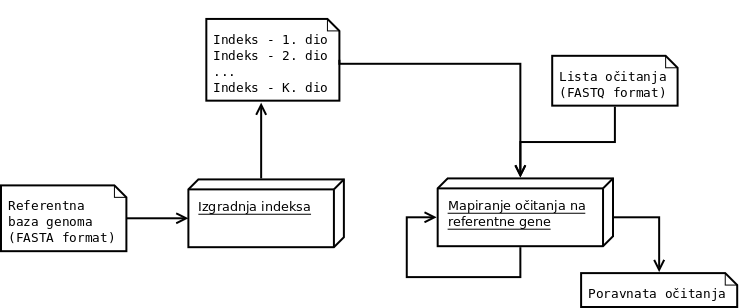
\includegraphics[width=1\textwidth]{../img/Komponente.png}
	\caption{Dijagram komponenata s njihovih ulazima/izlazima}
\end{center}
\end{figure}


Ostatak poglavlja će detaljnije obraditi pojedine komponente opisanog algoritma te njihove ulazne/izlazne podatke.

\section{Priprema podataka}

\section{Izgradnja indeksa}
\section{Mapiranje podataka}
\section{Paralelizacija algoritma}

\chapter{Rezultati}
U ovoj sekciji analiziramo performanse LISA-e. Analiza se provodi poravnanjem nad poznatim vrstama bakterija - kuga, salmonela, streptokok i E. Coli. Motivacija iza preciznog poravnanja očitanja u genome bakterije je jasna - efikasno i točno određivanje primjerice mutacija omogućuje brži dizajn lijekova za bakterije koje su stekle otpornost na postojeće lijekove.\\
Dajemo usporedbu LISA-e sa nekoliko modernih mappera. Uspoređujemo točnost i brzinu sa BWA-SW, BWA-MEM, SNAP i SeqAlto mapperom. Testna očitanja su generirana alatom za simuliranje wgsim koji je široko prihvaćen u bioinformatičkim krugovima i korišten u većini usporedbi.

\section {E. Coli}

\section {Salmonella Enterica}

\section {Streptococcus Pneumoniae}

\section {Yersinia Pestis}

\chapter{Zaključak i daljnji rad}
Zaključak.

\chapter{Dodatak}

\bibliography{literatura}
\bibliographystyle{fer}

\begin{sazetak}
Sažetak na hrvatskom jeziku.

\kljucnerijeci{Ključne riječi, odvojene zarezima.}
\end{sazetak}

% TODO: Navedite naslov na engleskom jeziku.
\engtitle{Title}
\begin{abstract}
Abstract.

\keywords{Keywords.}
\end{abstract}

\end{document}
